\chapter{Fonctions de référence}

\section{Parité d'une fonction}

\begin{defin}[Fonction paire, fonction impaire]
	Soit $f$ une fonction définie sur un ensemble $D$ symétrique par rapport à $0$.
	\begin{itemize}
		\item $f$ est \textbf{paire} si, pour tout $x \in D$, $f(-x) = f(x)$.
		\item $f$ est \textbf{impaire} si, pour tout $x \in D$, $f(-x) = -f(x)$.
	\end{itemize}

	\begin{center}
		\begin{tikzpicture}[scale=0.8]
			% Paire
			\begin{scope}[xshift=-5.5cm]
				\draw[very thin, gray!40] (-2.9,-0.5) grid (2.9,4.5);
				\draw[-{Stealth}, black, thick] (-3,0) -- (3,0) node[right] {$x$};
				\draw[-{Stealth}, black, thick] (0,-0.5) -- (0,4.5) node[above] {$y$};
				\draw[blue, ultra thick, domain=-2.1:2.1, samples=60] plot(\x, {\x*\x});
				\draw[dashed, red, thick] (0,-0.5) -- (0,4.5);
				\node[below] at (0,-0.7) {Courbe symétrique par rapport à $(Oy)$};
				\node[below, font=\bfseries] at (0,-1.3) {Fonction paire};
			\end{scope}
			% Impaire
			\begin{scope}[xshift=5.5cm,yshift=2cm]
				\draw[very thin, gray!40] (-2.9,-2.5) grid (2.9,2.5);
				\draw[-{Stealth}, black, thick] (-3,0) -- (3,0) node[right] {$x$};
				\draw[-{Stealth}, black, thick] (0,-2.5) -- (0,2.5) node[above] {$y$};
				\draw[green!50!black, ultra thick, domain=-1.6:1.6, samples=60] plot(\x, {0.6*\x*\x*\x});
				\filldraw[red] (0,0) circle (2.5pt);
				\node[below] at (0,-2.7) {Courbe symétrique par rapport à $O$};
				\node[below, font=\bfseries] at (0,-3.3) {Fonction impaire};
			\end{scope}
		\end{tikzpicture}
	\end{center}
\end{defin}

\begin{methode}[Démontrer la parité d'une fonction]
	\nline
	\begin{enumerate}
		\item \textbf{Fonction paire :} Démontrer que $f(x) = 5x^2 + 3$ est paire sur $\mathbb{R}$.
		\item \textbf{Fonction impaire :} Démontrer que $g(x) = x^3 - 3x$ est impaire sur $\mathbb{R}$.
	\end{enumerate}

	\begin{correction}
		\nline
		\begin{enumerate}
			\item Pour tout $x \in \mathbb{R}$, $-x \in \mathbb{R}$ :
			      \[
				      f(-x) = 5(-x)^2 + 3 = 5x^2 + 3 = f(x)
			      \]
			      Donc $f$ est \textbf{paire}. Sa courbe est symétrique par rapport à l'axe des ordonnées.

			\item Pour tout $x \in \mathbb{R}$, $-x \in \mathbb{R}$ :
			      \[
				      g(-x) = (-x)^3 - 3(-x) = -x^3 + 3x = -(x^3 - 3x) = -g(x)
			      \]
			      Donc $g$ est \textbf{impaire}. Sa courbe est symétrique par rapport à l'origine $O$.
		\end{enumerate}
	\end{correction}
\end{methode}

\newpage

\section{Fonctions de référence}

\subsection{Fonction carré}

\begin{defin}[Fonction carré]
	La \textbf{fonction carré} est la fonction $f$ définie sur $\mathbb{R}$ par :
	\[
		f(x) = x^2
	\]
\end{defin}

\begin{prop}[Propriétés et variations]
	\nline
	\begin{itemize}
		\item Pour tout $x \in \mathbb{R}$, $x^2 \ge 0$.
		\item La fonction carré est \textbf{paire}.
		\item Elle est strictement décroissante sur $] - \infty\,;\,0]$ et strictement croissante sur $[0\,;\, + \infty[$.
	\end{itemize}

	\begin{center}
		\begin{tikzpicture}
			\tkzTabInit[lgt=2, espcl=3]{$x$ / 0.5, $x^2$ / 1.5}{$-\infty$, $0$, $+\infty$}
			\tkzTabVar{+ / $+\infty$, - / $0$, + / $+\infty$}
		\end{tikzpicture}
	\end{center}
\end{prop}

\begin{prop}[Représentation graphique]
	La représentation graphique de la fonction carré est une \textbf{parabole} de sommet $O(0\,;\,0)$, symétrique par rapport à l'axe des ordonnées.

	\begin{center}
		\begin{tikzpicture}[scale=0.9]
			\draw[very thin, gray!40] (-3.5,-0.5) grid (3.5,4.5);
			\draw[-{Stealth}, black, thick] (-3.5,0) -- (3.5,0) node[right] {$x$};
			\draw[-{Stealth}, black, thick] (0,-0.5) -- (0,4.5) node[above] {$y$};
			\foreach \x in {-3,-2,-1,1,2,3} \node[below, font=\small] at (\x,0) {$\x$};
			\foreach \y in {1,2,3,4} \node[left, font=\small] at (0,\y) {$\y$};
			\draw[blue, ultra thick, domain=-2.1:2.1, samples=80] plot(\x, {\x*\x});
			\filldraw (0,0) circle (3pt);
			\filldraw (-2,4) circle (3pt) (-1,1) circle (3pt) (1,1) circle (3pt) (2,4) circle (3pt);
		\end{tikzpicture}
	\end{center}
\end{prop}

\begin{methode}[Résolution de l'équation $x^2 = k$]
	Pour résoudre dans $\mathbb{R}$ l'équation $x^2 = k$ :
	\begin{itemize}
		\item Si $k > 0$, l'équation possède \textbf{deux solutions} : $x = \sqrt{k}$ et $x = -\sqrt{k}$.
		\item Si $k = 0$, l'équation possède \textbf{une unique solution} : $x = 0$.
		\item Si $k < 0$, l'équation ne possède \textbf{aucune solution} dans $\mathbb{R}$.
	\end{itemize}

	\begin{ex}
		Résoudre dans $\mathbb{R}$ l'équation $x^2 = 144$.

		\begin{correction}
			Comme $144 > 0$, l'équation admet deux solutions : $\begin{cases} x = \sqrt{144} = 12 \\ x = -\sqrt{144} = -12 \end{cases}$

			Ainsi, $S = \{-12\,;\,12\}$.
		\end{correction}
	\end{ex}
\end{methode}

\newpage

\subsection{Fonction racine carrée}

\begin{defin}[Fonction racine carrée]
	La \textbf{fonction racine carrée} est la fonction $f$ définie sur $[0\,;\, + \infty[$ par :
	\[
		f(x) = \sqrt{x}
	\]
\end{defin}

\begin{prop}[Variations et courbe]
	La fonction racine carrée est \textbf{strictement croissante} sur $[0\,;\, + \infty[$.

	Sa représentation graphique est une demi-parabole observée sur $[0\,;\, + \infty[$.

	\begin{center}
		\begin{tabular}{ccc}
			\begin{tikzpicture}[baseline=(current bounding box.center)]
				\tkzTabInit[lgt=1.8, espcl=2.5]{$x$ / 0.75, $\sqrt{x}$ / 1.5}{$0$, $+\infty$}
				\tkzTabVar{- / $0$, + /$+\infty$ }
			\end{tikzpicture}
			 & ~\hspace{2cm}~ &
			\begin{tikzpicture}[scale=0.8,baseline=(current bounding box.center)]
				\draw[very thin, gray!40] (-0.5,-0.5) grid (5.5,3.5);
				\draw[-{Stealth}, black, thick] (-0.5,0) -- (5.5,0) node[right] {$x$};
				\draw[-{Stealth}, black, thick] (0,-0.5) -- (0,3.5) node[above] {$y$};
				\foreach \x in {1,2,3,4,5} \node[below, font=\small] at (\x,0) {$\x$};
				\foreach \y in {1,2,3} \node[left, font=\small] at (0,\y) {$\y$};
				\draw[orange!90!black, ultra thick, domain=0:5.2, samples=100] plot(\x, {sqrt(\x)});
				\filldraw (0,0) circle (3pt);
				\filldraw (1,1) circle (3pt) (4,2) circle (3pt);
			\end{tikzpicture}
		\end{tabular}
	\end{center}
\end{prop}

\begin{methode}[Résoudre une équation de la forme $\sqrt{A(x)} = k$]
	Pour résoudre dans $\mathbb{R}$ l'équation $\sqrt{A(x)} = k$ :
	\begin{itemize}
		\item Si $k < 0$, l'équation n'a \textbf{aucune solution} ($S = \emptyset$) car une racine carrée est toujours positive ou nulle.
		\item Si $k \ge 0$, l'équation équivaut à $A(x) = k^2$, sous réserve que $A(x) \ge 0$.
	\end{itemize}
\end{methode}

\begin{ex}
	Résoudre dans $\mathbb{R}$ les équations :
	\begin{multicols}{3}
		\begin{enumerate}
			\item $\sqrt{x + 2} = -3$
			\item $\sqrt{2x - 1} = 5$
		\end{enumerate}
	\end{multicols}

	\begin{correction}
		\nline
		\begin{enumerate}
			\item Pour que la racine carrée soit définie, le terme sous la racine doit être supérieur ou égal à $0$ :
			      \[
				      x + 2 \ge 0 \iff x \ge -2
			      \]
			      Le membre de gauche est donc positif ou nul pour tout $x \ge -2$.

			      Or, le membre de droite est strictement négatif ($-3 < 0$).

			      Une racine carrée ne pouvant jamais être égale à un nombre négatif, l'équation n'a pas solution : $S = \emptyset$.

			\item Pour que la racine carrée soit définie, l'expression sous le radical doit être supérieur ou égal à $0$ :
			      \begin{align*}
				      2x - 1 \ge 0 & \iff 2x \ge 1          \\
				                   & \iff x \ge \frac{1}{2}
			      \end{align*}

			      Le membre de droite étant positif ($5 \ge 0$), on peut élever au carré sur l'intervalle $\left[ \dfrac{1}{2}\,;\, + \infty \right[$ :
			      \begin{align*}
				      \sqrt{2x - 1} = 5 & \iff 2x - 1 = 5^2 \\
				                        & \iff 2x - 1 = 25  \\
				                        & \iff 2x = 26      \\
				                        & \iff x = 13
			      \end{align*}

			      Comme $13 \ge \frac{1}{2}$, la solution est valide. Ainsi, $S = \brac{13}$.
		\end{enumerate}
	\end{correction}
\end{ex}

\newpage

\subsection{Fonction inverse}

\begin{defin}[Fonction inverse]
	La \textbf{fonction inverse} est la fonction $f$ définie sur $\mathbb{R} \setminus \{0\}$ (ou $\mathbb{R}^*$) par :
	\[
		f(x) = \dfrac{1}{x}
	\]
\end{defin}

\begin{prop}[Propriétés et variations]
	\nline
	\begin{itemize}
		\item La fonction inverse est \textbf{impaire}.
		\item Elle est \textbf{strictement décroissante} sur $] - \infty\,;\,0[$ et \textbf{strictement décroissante} sur $]0\,;\, + \infty[$.
	\end{itemize}

	\begin{center}
		\begin{tikzpicture}
			\tkzTabInit[lgt=2, espcl=2.5]{$x$ / 0.5, $\dfrac{1}{x}$ / 1.5}{$-\infty$, $0$, $+\infty$}
			\tkzTabVar{+ / $0$ , -D+ / $-\infty$ / $+\infty$ , - / $0$ }
		\end{tikzpicture}
	\end{center}
\end{prop}

\begin{prop}[Représentation graphique]
	La représentation graphique de la fonction inverse est une \textbf{hyperbole}, admettant l'origine $O(0\,;\,0)$ comme centre de symétrie.
	\begin{center}
		\begin{tikzpicture}[scale=0.8]
			\draw[very thin, gray!40] (-4.5,-3.5) grid (4.5,3.5);
			\draw[-{Stealth}, black, thick] (-4.5,0) -- (4.5,0) node[right] {$x$};
			\draw[-{Stealth}, black, thick] (0,-3.5) -- (0,3.5) node[above] {$y$};
			\foreach \x in {-4,-3,-2,-1,1,2,3,4} \node[below, font=\small] at (\x,0) {$\x$};
			\foreach \y in {-3,-2,-1,1,2,3} \node[left, font=\small] at (0,\y) {$\y$};
			\draw[magenta, ultra thick, domain=-4.2:-0.30, samples=100] plot(\x, {1/\x});
			\draw[magenta, ultra thick, domain=0.30:4.2, samples=100] plot(\x, {1/\x});
			\filldraw (0,0) circle (3pt);
			\filldraw (-1,-1) circle (3pt) (1,1) circle (3pt);
		\end{tikzpicture}
	\end{center}
\end{prop}

\begin{methode}[Calcul d'image et d'antécédent]
	Soit $f$ la fonction définie sur $\mathbb{R}^*$ par $f(x) = 2 + \dfrac{3}{x}$.
	\begin{enumerate}
		\item Calculer l'image de $3$ par $f$.
		\item Déterminer l'antécédent de $7$ par $f$.
	\end{enumerate}

	\begin{correction}
		\nline
		\begin{enumerate}
			\item $f(3) = 2 + \dfrac{3}{3} = 2 + 1 = 3$.

			      L'image de $3$ est $3$.
			\item On résout $f(x) = 7$ :
			      \begin{align*}
				      2 + \frac{3}{x} = 7 & \iff \frac{3}{x} = 5                   \\
				                          & \iff 5x = 3 \quad \iff x = \frac{3}{5}
			      \end{align*}
			      L'antécédent de $7$ par $f$ est $\dfrac{3}{5}$.
		\end{enumerate}
	\end{correction}
\end{methode}

\newpage

\subsection{Fonction cube}

\begin{defin}[Fonction cube]
	La \textbf{fonction cube} est la fonction $f$ définie sur $\mathbb{R}$ par :
	\[
		f(x) = x^3
	\]
\end{defin}

\begin{prop}[Variations et courbe]
	La fonction cube est \textbf{impaire} et \textbf{strictement croissante} sur $\mathbb{R}$.

	Sa courbe est symétrique par rapport à l'origine $O(0\,;\,0)$.

	\begin{center}
		\begin{tabular}{ccc}
			\begin{tikzpicture}[baseline=(current bounding box.center)]
				\tkzTabInit[lgt=1.8, espcl=2.5]{$x$ / 0.5, $x^3$ / 1.5}{$-\infty$, $+\infty$}
				\tkzTabVar{- / $-\infty$ , + / $+\infty$}
			\end{tikzpicture}
			 & ~\hspace{2cm}~ &
			\begin{tikzpicture}[scale=0.75,baseline=(current bounding box.center)]
				\draw[very thin, gray!40] (-3.5,-3.5) grid (3.5,3.5);
				\draw[-{Stealth}, black, thick] (-3.5,0) -- (3.5,0) node[right] {$x$};
				\draw[-{Stealth}, black, thick] (0,-3.5) -- (0,3.5) node[above] {$y$};
				\foreach \x in {-3,-2,-1,1,2,3} \node[below, font=\small] at (\x,0) {$\x$};
				\foreach \y in {-3,-2,-1,1,2,3} \node[left, font=\small] at (0,\y) {$\y$};
				\draw[green!60!black, ultra thick, domain=-1.5:1.5, samples=80] plot(\x, {\x*\x*\x});
				\filldraw (0,0) circle (3pt);
				\filldraw (-1,-1) circle (3pt) (1,1) circle (3pt);
			\end{tikzpicture}
		\end{tabular}
	\end{center}
\end{prop}

\section{Positions relatives des courbes}

\begin{prop}[Comparaison sur $\intfo{0}{+\infty}$]
	Pour tout $x \ge 0$, les positions relatives des courbes d'équations $y = x$, $y = x^2$ et $y = x^3$ dépendent de la position de $x$ par rapport à $1$ :
	\begin{itemize}
		\item Si $0 \le x \le 1$, alors $x^3 \le x^2 \le x$.
		\item Si $x \ge 1$, alors $x \le x^2 \le x^3$.
	\end{itemize}

	\begin{center}
		\begin{tikzpicture}[x=3cm,y=3cm]
			\draw[very thin, gray!40,step=0.5] (-0.1,-0.1) grid (2.2,2.45);
			\draw[-{Stealth}, black, thick] (-0.2,0) -- (2.2,0) node[right] {$x$};
			\draw[-{Stealth}, black, thick] (0,-0.2) -- (0,2.5) node[above] {$y$};
			\draw[dashed, red, thick] (1,-0.2) -- (1,2.5);
			\draw[red, very thick, domain=0:2.1] plot(\x, {\x}) node[right, font=\large] {$y = x$};
			\draw[blue, very thick, domain=0:1.58, samples=100] plot(\x, {\x*\x}) node[right, font=\large] {$y = x^2$};
			\draw[green!60!black, very thick, domain=0:1.35, samples=100] plot(\x, {\x*\x*\x}) node[above, font=\large] {$y = x^3$};
			\draw[dotted, gray!70, very thick, domain=0:2.1, samples=100] plot(\x, {sqrt(\x)}) node[right, font=\large] {$y = \sqrt{x}$};
			\filldraw (0,0) circle (3pt) (1,1) circle (3pt);
			\node[below] at (0.5,-0.2) {$0 \le x \le 1$};
			\node[below] at (1.5,-0.2) {$x \ge 1$};
			\node[below left] at (0,0) {$0$};
			\node[below, fill=white] at (1,-0.05) {$1$};
			\node[below, fill=white] at (2,-0.05) {$2$};
			\node[left, fill=white] at (-0.05,1) {$1$};
			\node[left, fill=white] at (-0.05,2) {$2$};
		\end{tikzpicture}
	\end{center}
\end{prop}

\newpage

\begin{demo}[Positions relatives]
	\nline
	\begin{itemize}[itemsep=2mm]
		\item \emph{\textbf{Cas 1 : $x \ge 1$}}
		      \begin{itemize}[itemsep=1mm]
			      \item Signe de $x^2 - x = x(x - 1)$ :

			            Comme $x \ge 0$ et $x - 1 \ge 0$, $x^2 - x \ge 0$, donc la courbe $y = x^2$ est \textbf{au-dessus} de $y = x$.
			      \item Signe de $x^3 - x^2 = x^2(x - 1)$ :

			            Comme $x^2 \ge 0$ et $x - 1 \ge 0$, $x^3 - x^2 \ge 0$, donc la courbe $y = x^3$ est \textbf{au-dessus} de $y = x^2$.
		      \end{itemize}

		\item \emph{\textbf{Cas 2 : $0 \le x \le 1$}}
		      \begin{itemize}[itemsep=1mm]
			      \item Signe de $x^2 - x = x(x - 1)$ :

			            Comme $x \ge 0$ et $x - 1 \le 0$, $x^2 - x \le 0$, donc la courbe $y = x^2$ est \textbf{en dessous} de $y = x$.
			      \item Signe de $x^3 - x^2 = x^2(x - 1)$ :

			            Comme $x^2 \ge 0$ et $x - 1 \le 0$, $x^3 - x^2 \le 0$, donc la courbe $y = x^3$ est \textbf{en dessous} de $y = x^2$.
		      \end{itemize}
	\end{itemize}
\end{demo}

\section{Tableaux de signes des fonctions de référence}

\begin{center}
	\def\arraystretch{1.4}
	\begin{tabular}{|c|c|c|} \hline
		\textbf{Fonction}                               & \textbf{Domaine}    & \textbf{Tableau de signes} \\ \hline
		\rule[-10mm]{0mm}{20mm}$x \mapsto x^2$          & $\mathbb{R}$        &
		\begin{tikzpicture}[baseline=(current bounding box.center)]
			\tkzTabInit[lgt=1.2, espcl=1.5]{$x$/0.8, $x^2$/0.8}{$-\infty$, $0$, $+\infty$}
			\tkzTabLine{,+,z,+,}
		\end{tikzpicture} \\ \hline
		\rule[-10mm]{0mm}{20mm}$x \mapsto \sqrt{x}$     & $[0\,;\, + \infty[$ &
		\begin{tikzpicture}[baseline=(current bounding box.center)]
			\tkzTabInit[lgt=1.2, espcl=1.5]{$x$/0.8, $\sqrt{x}$/0.8}{$0$, $+\infty$}
			\tkzTabLine{z,+,}
		\end{tikzpicture} \\ \hline
		\rule[-10mm]{0mm}{20mm}$x \mapsto \dfrac{1}{x}$ & $\mathbb{R}^*$      &
		\begin{tikzpicture}[baseline=(current bounding box.center)]
			\tkzTabInit[lgt=1.2, espcl=1.5]{$x$/0.8, $\frac{1}{x}$/0.8}{$-\infty$, $0$, $+\infty$}
			\tkzTabLine{,-,d,+,}
		\end{tikzpicture} \\ \hline
		\rule[-10mm]{0mm}{20mm}$x \mapsto x^3$          & $\mathbb{R}$        &
		\begin{tikzpicture}[baseline=(current bounding box.center)]
			\tkzTabInit[lgt=1.2, espcl=1.5]{$x$/0.8, $x^3$/0.8}{$-\infty$, $0$, $+\infty$}
			\tkzTabLine{,-,z,+,}
		\end{tikzpicture} \\ \hline
	\end{tabular}
\end{center}

